\documentclass[11pt]{article}

%%% PAGE DIMENSIONS
\usepackage{geometry}
\geometry{a4paper}

%%% PACKAGES
\usepackage[english]{babel}
\usepackage[utf8]{inputenc}
\usepackage{graphicx}
\usepackage[parfill]{parskip}
\usepackage{booktabs}
\usepackage{array}
\usepackage{paralist}
\usepackage{verbatim}
\usepackage{subfig}
\usepackage{cite}
\usepackage{amsmath}
\usepackage[colorinlistoftodos]{todonotes}

%%% IMAGE FILES PATH
\graphicspath{{Images/}}

%%% HEADERS & FOOTERS
\usepackage{fancyhdr}
\pagestyle{fancy}
\renewcommand{\headrulewidth}{0pt}
\lhead{}\chead{}\rhead{}
\lfoot{}\cfoot{\thepage}\rfoot{}

%%% SECTION TITLE APPEARANCE
\usepackage{sectsty}
\allsectionsfont{\sffamily\mdseries\upshape}

%%% TABLE OF CONTENTS APPEARANCE
\usepackage[nottoc,notlof,notlot]{tocbibind}
\usepackage[titles,subfigure]{tocloft}
\renewcommand{\cftsecfont}{\rmfamily\mdseries\upshape}
\renewcommand{\cftsecpagefont}{\rmfamily\mdseries\upshape}

%%% DOCUMENT
\title{Mapping the Brain: An Introduction to Connectomics\\Streamlining Analysis for Automated Neuronal Membrane Segmentation Pipelines}

\author{Thomas Keady, Albert Lee, Augusto Ramirez}

\date{\today}

\begin{document}
\maketitle

\section{Abstract}

Creating a complete wiring diagram of neuronal connectivity is one of the most ambitious goals of connectomics and contemporary neuroscience \cite{roncal1}. Thanks to technical and computational advances that automate the collection of high resolution electron-microscopy data, complex networks of neurons and their synaptic connections can be directly observed and eventually fully mapped. An important step in this process is the annotation of membranes, which allows for deeper levels of analysis. However, the most reliable method of membrane detection to date is performed manually \cite{plaza}. Although automated membrane segmentation tools exist, the landscape of such algorithms consists mainly of poor documentation and untested parameters/optimization. The neuroXplorer team ran tested popular image processing functions such as watershed and gala in different testing environments (Matlab, Python) \cite{nguyen}.

By comparing a range of parameters on a set of images, relevant statistical data can be inferred and utilized to select the arguments needed to optimize the tools mentioned earlier. Reducing the average error rates for metrics such as split\_VI, adjusted rand index, and Fowlkes-Mallows index can help us indicate optimized parameters for each image.

\section{Results}

Three parameters within our program were varied to find their optimal values. These were the size of the closing footprint, the size of the median filter, and the size of the watershed footprint. To obtain the ideal parameters, we tested a sparse but evenly distributed sampling of the possible combinations of values on our training dataset. We then found the parameters that led to the most similar segmentation to ground truth according to four metrics: the rate of under segmentation (merge errors), the rate of over segmentation (split errors), the adjusted rand index, and the Fowlkes-Mallows index. For each image, we recorded the parameters that led to the best segmentation according to each of the four metrics. We then used the resulting ranges of parameters to do a narrow, more denser sweep to more finely tune the parameters. After again identifying the best segmentations and their corresponding parameters, we averaged each parameter and rounded to the nearest integer to get our final parameters. The size of the closing footprint became 24, the size of the median filter was 7, and the size of the watershed footprint was 1. Across all metrics the optimized parameters were very close to each other, +/- 1. There was one exception: the undersegmentation metric was best optimized when the watershed footprint was 6 (6.07 averaged), while all three other metrics optimized it to 1.00 exactly. We decided to use the optimized parameter as 1 instead of averaging three 1's with a 6, and applied these parameters to our testing dataset. All of the metrics appeared similar between the training and testing datasets. We had slightly better segmentations in the training set, according to the graphs on our poster. We speculate that this was due to underfitting, where the algorithm was not subjected to enough possible cases to optimize its parameters as best as possible, rather than overfitting where its optimization became so tailored to the training set such that it did not extrapolate well. We primarily believe this because of the relatively small size of our training set (50 sections). Also, in both the training and testing datasets, the algorithm was prone to oversegmentation as can be seen in our graphs and images. However, we point out that our algorithm does considerably better with merge errors, and believe this is valuable as merge errors are more difficult to rectify than split errors. 

\begin{figure}
	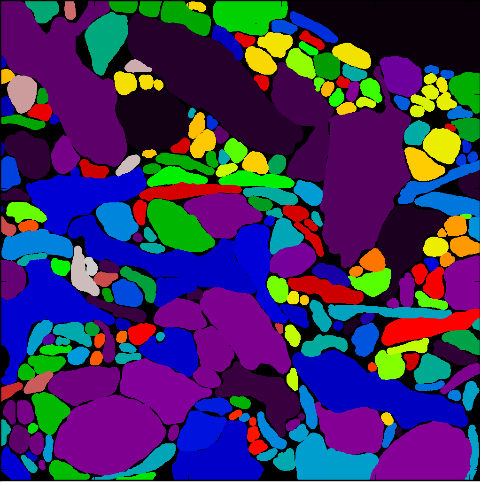
\includegraphics{truth_anno1}
	\caption{Fully annotated ground truth.}
\end{figure}

\begin{figure}
	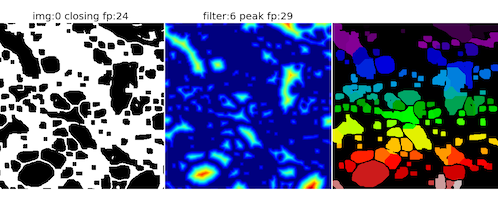
\includegraphics{fig_0_24_6_29}
	\caption{Watershed optimized membrane segmentation.}
\end{figure}


\begin{thebibliography}{1}
\bibitem{roncal1} W. G. Roncal, D. M. Kleissas, J. T. Vogelstein, "An automated images-to-graphs pipeline for high resolution connectomics." \textit{Frontiers in Neuroinformatics}, vol. 9, no. 20, Aug. 2015.
\bibitem{plaza} S. Plaza, "Focused Proofreading: Efficiently Extracting Connectomes from Segmented EM Images." \textit{Cornell University Library}, Sep. 2014.
\bibitem{nguyen} Q. Nguyen,  "Parallel and scalable neural image segmentation for connectome graph extraction.” \textit{DSpace at MIT}. Aug. 2015.
\end{thebibliography}

\end{document}